
\documentclass{article}
\usepackage[T1]{fontenc}
\usepackage{graphicx}
\usepackage{amsmath, amsthm, amssymb}
\usepackage{hyperref}
\usepackage{polski}
\usepackage{minted}
\setminted[c]{breaklines}

\title{SPRAWOZDANIE - LISTA 3}
\author{Zuzanna Pawlik, 282230}
\date{09.01.2025}
\begin{document}
	\maketitle
	
	\section*{FRAGMENTY KODÓW}
	\subsection*{CUT ROD}
	Fragment kodu CUTROD w wersji naiwnej:
	\begin{minted}{c}
		int CUT_ROD(int p[], int n){
			if(n==0) return 0;
			
			int q = INT_MIN;
			for(int i = 1; i <= n; i++){
				q = max(q,p[i]+CUT_ROD(p,n-i));
			}
			return q;
		}
	\end{minted}
	Fragment kodu CUTROD w wersji ze spamiętywaniem: 
	\begin{minted}{c}
		int MEMORIZED_CUT_ROD(int p[], int r[], int s[], int n){
			if(r[n] >= 0) return r[n];
			int q;
			if(n==0){
				q = 0;
			}else{
				q = INT_MIN;
				for(int i = 1; i <= n; i++){
					int t = p[i] + MEMORIZED_CUT_ROD(p,r,s,n-i);
					if(q < t){
						q = t;
						s[n] = i;
					}
				}
				
			}
			r[n] = q;
			return q;
		}
		
	\end{minted}
	Fragment kodu CUTROD w wersji iteracyjnej:	
	\begin{minted}{c}
		void EXT_BOT_UP_CUT_ROD(int p[], int n, int r[], int s[]){
			r[0] = 0;
			
			for(int j = 1; j <= n; j++){
				int q = INT_MIN;
				for(int i = 1; i <= j; i++){
					if(q < p[i]+r[j-i]){
						q = p[i]+r[j-i];
						s[j] = i;
					}
				}
				r[j] = q;
			}
		}
	\end{minted}
	Zarówno wersja z zapamiętywaniem, jak i iteracyjna wykorzystują dodatkowo funkcje wypisujące rozwiązania, w których definiowane są również tablice pomocnicze $r$ i $s$.
	\subsection*{NAJDŁUŻSZY WSPÓLNY PODCIĄG}
	Fragment algorytmu LCS w wersji rekurencyjnej:
	\begin{minted}{c}
		int LCS_REK(const string &X, const string &Y, int m, int n, int **b){
			if(m==0 || n==0) return 0;
			if(b[m][n] != -1) return b[m][n]; //juz wpisane
			if(X[m-1] == Y[n-1]) return b[m][n] = 1 + LCS_REK(X,Y,m-1,n-1,b);//sprawdz ostatni
			return b[m][n] = max(LCS_REK(X,Y,m,n-1,b),LCS_REK(X,Y,m-1,n,b));//wynik    
		}
		
		void LCS_REK_SOLUTION(const string &X, const string &Y){
			int m = X.length();
			int n = Y.length();
			
			int **b = new int*[m+1];
			for(int i = 0; i<=m; i++){
				b[i] = new int[n+1];
				for(int j = 0; j <= n; j++){
					b[i][j] = -1;
				}
			}
			
			int k = LCS_REK(X,Y,m,n,b);
			
			string p = "";
			int i = m;
			int j = n;
			while(i > 0 && j > 0){
				if(X[i-1] == Y[j-1]){
					p = X[i-1]+p;
					i--;
					j--;
				}else if(b[i-1][j] > b[i][j-1]){
					i--;
				}else{
					j--;
				}
			}
			cout << "dlugosc podciagu: " << k << endl;
			cout << "podciag: " << p << endl;
			
			delete[] b;
			
		}
	\end{minted}
	Fragment algorytmu LCS w wersji iteracyjnej:
	\begin{minted}{c}
		char** LCS_ITEROWANE(string& X, string& Y, int& d){
			int m = X.length();
			int n = Y.length();
			
			char** b = new char*[m+1];
			int** c = new int*[m+1];
			
			for(int i = 0; i <= m; i++){
				b[i] = new char[n+1];
				c[i] = new int[n+1];
			}
			
			for(int j = 0; j<=m; j++){
				c[j][0] = 0;
			}
			for(int j = 0; j<=n; j++){
				c[0][j] = 0;
			}
			
			for(int i = 1; i <= m; i++){
				for(int j = 1; j <= n; j++){
					if(X[i-1] == Y[j-1]){
						c[i][j] = c[i-1][j-1]+1;
						b[i][j] = 's';
					}else if(c[i-1][j] >= c[i][j-1]){
						c[i][j] = c[i-1][j];
						b[i][j] = 'g';
					}else{
						c[i][j] = c[i][j-1];
						b[i][j] = 'l';
					}
				}
			}
			d = c[m][n];
			return b;
		}
		
		void PRINT_SOLUTION(char** b, string& X, int i, int j){
			if(i>0 && j>0){
				if(b[i][j] == 's'){
					PRINT_SOLUTION(b,X,i-1,j-1);
					cout << X[i - 1];
				}else if(b[i][j] == 'g'){
					PRINT_SOLUTION(b,X,i-1,j);
				}else{
					PRINT_SOLUTION(b,X,i,j-1);
				}
				
			}
		}
	\end{minted}
	Obie wersje pozwalają wyznaczyć najdłuższy wspólny podciąg dwóch napisów, a także długość takiego ciągu. W LCS iterowanym zamiast strzałek użyta jest notacja: $g$ - w górę, $l$ - w lewo oraz $s$ - na skos. Oba algorytmy wykorzystują dodatkowe funkcje pozwalające na wypisanie znalezionego ciągu.
	\subsection*{WYBÓR ZAJĘĆ}
	\subsubsection*{REKURENCJA}
	Algorytm rekurencyjny:
	\begin{minted}{c}
		void RECURSIVE_ACTIVITY_SELECTOR(int s[], int f[], int k, int n, int wyniki[], int& ilosc){
			int m = k+1;
			while(m<=n && s[m] < f[k]){
				m++;
			}
			
			if(m<=n){
				wyniki[ilosc++] = m;//dodajemy do zajęć
				RECURSIVE_ACTIVITY_SELECTOR(s,f,m,n,wyniki,ilosc);
			}
		}
		
		void PRINT_RAS(int s[], int f[], int n){
			int* wyniki = new int[n];
			int ilosc = 0;
			
			RECURSIVE_ACTIVITY_SELECTOR(s,f,0,n,wyniki,ilosc);
			cout << "rekurencja:" <<endl;
			for(int i = 0; i < ilosc; i++){
				cout << wyniki[i] << " ";
				
			}
			cout<<endl;
			
			
		}
	\end{minted}
	Modyfikacja:
	\begin{minted}{c}
		void RAS_MOD(Zajecia lista_zajec[], int k, int n, int wyniki[], int& ilosc) {
			int m = k + 1;
			while (m <= n && lista_zajec[m].poczatek < lista_zajec[k].koniec){
				m++;
			}
			
			if (m <= n){
				wyniki[ilosc++] = lista_zajec[m].index; 
				RAS_MOD(lista_zajec, m, n, wyniki, ilosc); 
			}
		}
		
		void PRINT_RAS_MOD(Zajecia lista_zajec[], int n){
			int wyniki[n];
			int ilosc = 0;
			
			RAS_MOD(lista_zajec, 0, n, wyniki, ilosc);
			cout << "rekurencja modyfikacja:" <<endl;
			for(int i = 0; i < ilosc; i++){
				cout << wyniki[i] << " ";
				
			}
			cout<<endl;    
		}
	\end{minted}
	\subsubsection*{ITERACJA}
	Algorytm iteracyjny:
	\begin{minted}{c}
		void ACTIVITY_SELECTOR(int s[], int f[], int n, int wyniki[], int& ilosc){
			int k = 1;//poczatek
			wyniki[ilosc++] = 1;//pierwsze zajecia
			
			for(int m = 2; m <= n; m++){
				if(s[m] >= f[k]){
					wyniki[ilosc++] = m;
					k = m;
				}
			}
			
		}
		
		void PRINT_AS(int s[], int f[], int n){
			int wyniki[n];
			int ilosc = 0;
			
			ACTIVITY_SELECTOR(s,f,n,wyniki,ilosc);
			
			cout << "iteracyjna:"<<endl;
			for(int i = 0; i<ilosc; i++){
				cout << wyniki[i] << " ";
				
			}
			cout << endl;
		}
	\end{minted}
	Modyfikacja:
	\begin{minted}{c}
		void AS_MOD(Zajecia lista_zajec[], int n, int wyniki[], int& ilosc){
			wyniki[ilosc++] = lista_zajec[1].index;
			int k = 1;
			
			for(int m = 2; m<=n; m++){
				if(lista_zajec[m].poczatek >= lista_zajec[k].koniec){
					wyniki[ilosc++] = lista_zajec[m].index;
					k = m;
				}
			}
		}
		
		void PRINT_AS_MOD(Zajecia lista_zajec[], int n){
			int wyniki[n];
			int ilosc = 0;
			
			AS_MOD(lista_zajec,n,wyniki,ilosc);
			
			cout << "iteracja modyfikacja:" <<endl;
			for(int i = 0; i < ilosc; i++){
				cout << wyniki[i] << " ";
				
			}
			cout<<endl; 
		}
	\end{minted}
	Modyfikacje powyższych algorytmów wykorzystują strukturę $Zajecia$, dla której określamy $poczatek$ - czas rozpoczęcia, $koniec$ - czas zakończenia oraz $index$ - początkową pozycję zajęć. Następnie takie zajęcia sortowane są po czasie rozpoczęcia i dopiero następuje wybór optymalnej opcji.
	\subsubsection*{PROGRAMOWANIE DYNAMICZNE}
	Wersja algorytmu wykorzystująca programowanie dynamiczne:
	\begin{minted}{c}
		void AS_DYNAM(int s[], int f[], int n){
			int max_zajec[n];  
			int poprzedni[n];  
			
			for (int i = 0; i < n; i++){
				max_zajec[i] = 1;
				poprzedni[i] = -1;
			}
			
			for (int i = 1; i < n; i++){
				for (int j = 0; j < i; j++){
					if (f[j] <= s[i]){
						if (max_zajec[j] + 1 > max_zajec[i]){//sprawdzenie czy wiecej zajec
							max_zajec[i] = max_zajec[j] + 1;
							poprzedni[i] = j;
						}
					}
				}
			}
			
			
			int index_max = 0;
			for (int i = 1; i < n; i++){
				if (max_zajec[i] > max_zajec[index_max]){//wybor maksymalnego zestawu
					index_max = i;
				}
			}
			
			
			int wynik[n];
			int ilosc = 0;
			
			while (index_max != -1){
				wynik[ilosc++] = index_max + 1;
				index_max = poprzedni[index_max];
			}
			
			
			cout << "prog. dynamiczne: ";
			for (int i = ilosc - 1; i >= 0; i--){
				cout << wynik[i] << " ";
			}
			cout << endl;
		}
	\end{minted}
	Kod ten przy pomocy tabel $max_zajec$ oraz $poprzedni$ pozwala znaleźć optymalne rozwiązanie dla tego problemu. W podwójnej pętli $for$ sprawdzane są zajęcia $i$ względem wcześniejszych zajęć $j$. Ostatecznie wyznaczany jest $index_max$, czyli indeks, dla którego $max_zajec[index_max]$ jest największe, a zatem optymalne rozwiązanie.
	\section*{TABELE I WYKRESY}
	\subsection*{PORÓWNANIE ALGORYTMÓW CUTROD}
	\begin{center}
		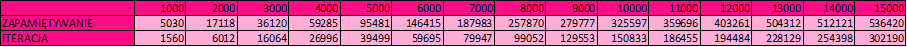
\includegraphics[width = \textwidth]{Obraz8.png}
	\end{center}
	\begin{center}
		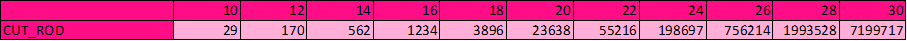
\includegraphics[width = \textwidth]{Obraz7.png}
	\end{center}
	\begin{center}
		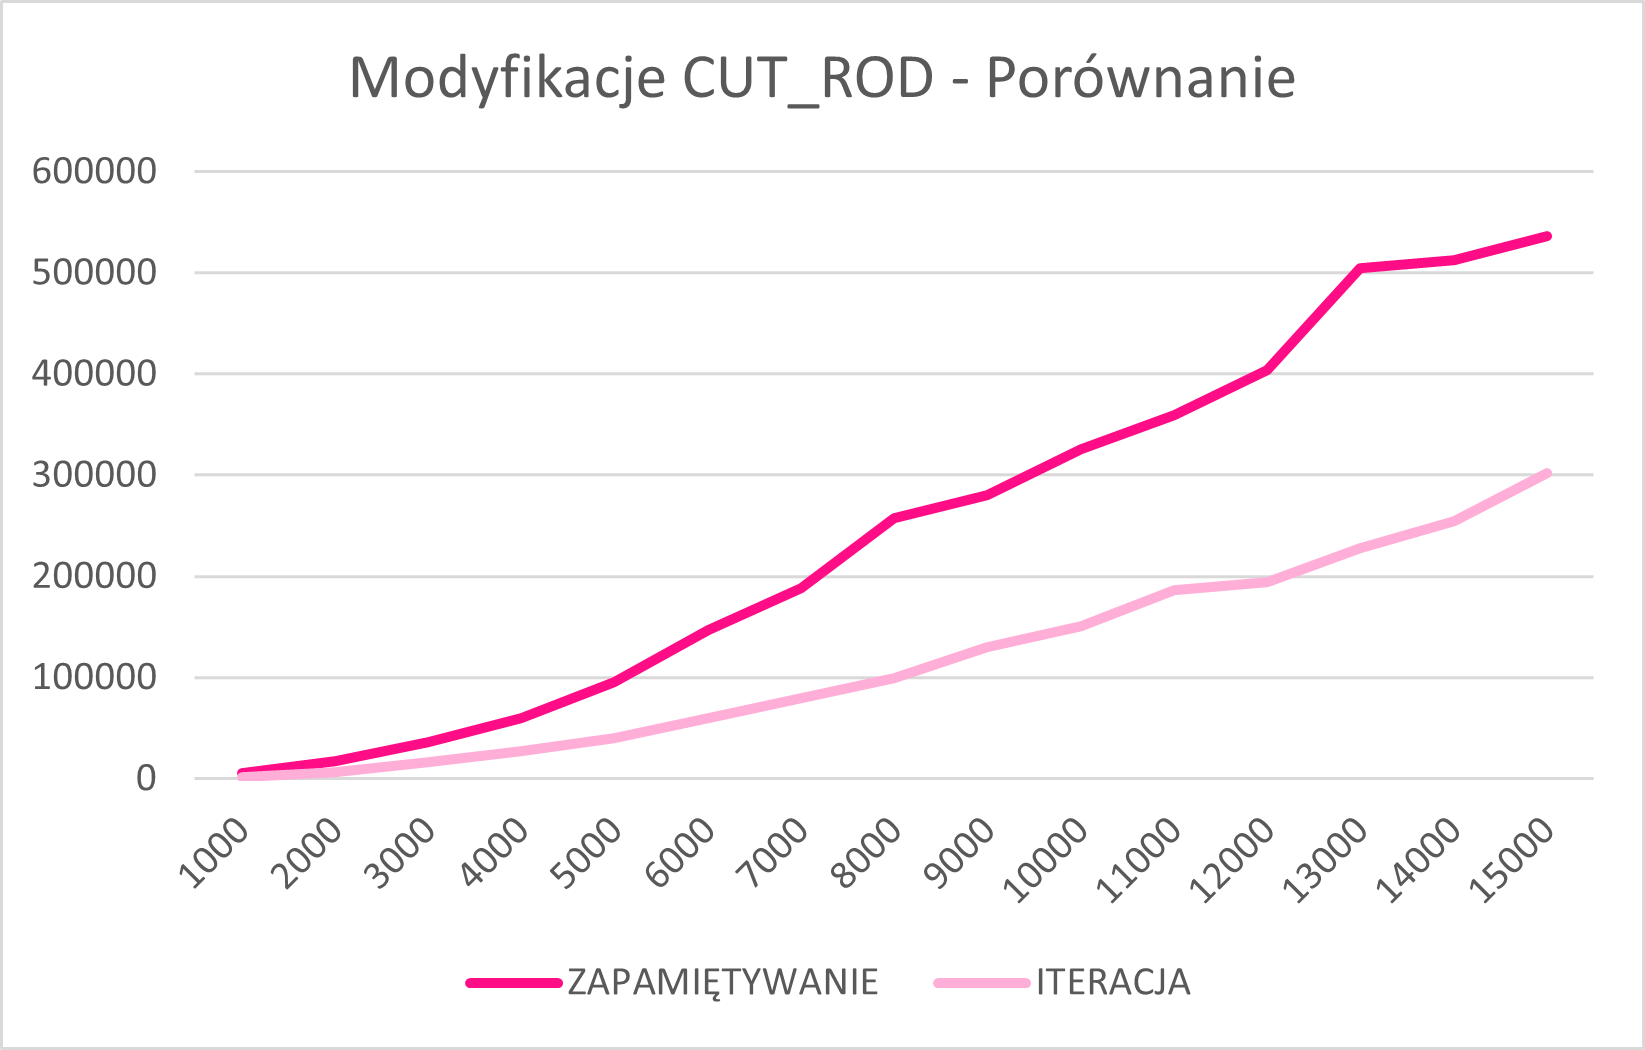
\includegraphics[width = \textwidth]{Obraz3.png}
	\end{center}
	\section*{WNIOSKI}
	Powyższe porównanie pozwala stwierdzić, że najbardziej wydajną wersją tego algorytmu jest ta, wykorzystująca iterację. Jest ona zauważalnie szybsza od algorytmu rekurencyjnego, choć oba wykonują się raczej sprawnie w porównaniu z wersją naiwną. Niestety, dokładne zaobserwowanie tej różnicy okazało się niemożliwe, ponieważ zwykły CUTROD już na małych danych wykonywał się znacznie dłużej od pozostałych dwóch. Dla tak małych długości pomiar "lepszych" wersji algorytmu okazał się po prostu niemożliwy, natomiast warunki sprzętowe nie pozwoliły na próbę sprawdzenia algorytmu naiwnego na dużych danych.
	\subsection*{PORÓWNANIE ALGORYTMÓW LCS}
	\begin{center}
		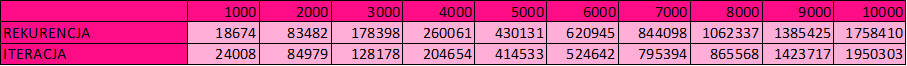
\includegraphics[width = \textwidth]{Obraz6.png}
	\end{center}
	\begin{center}
		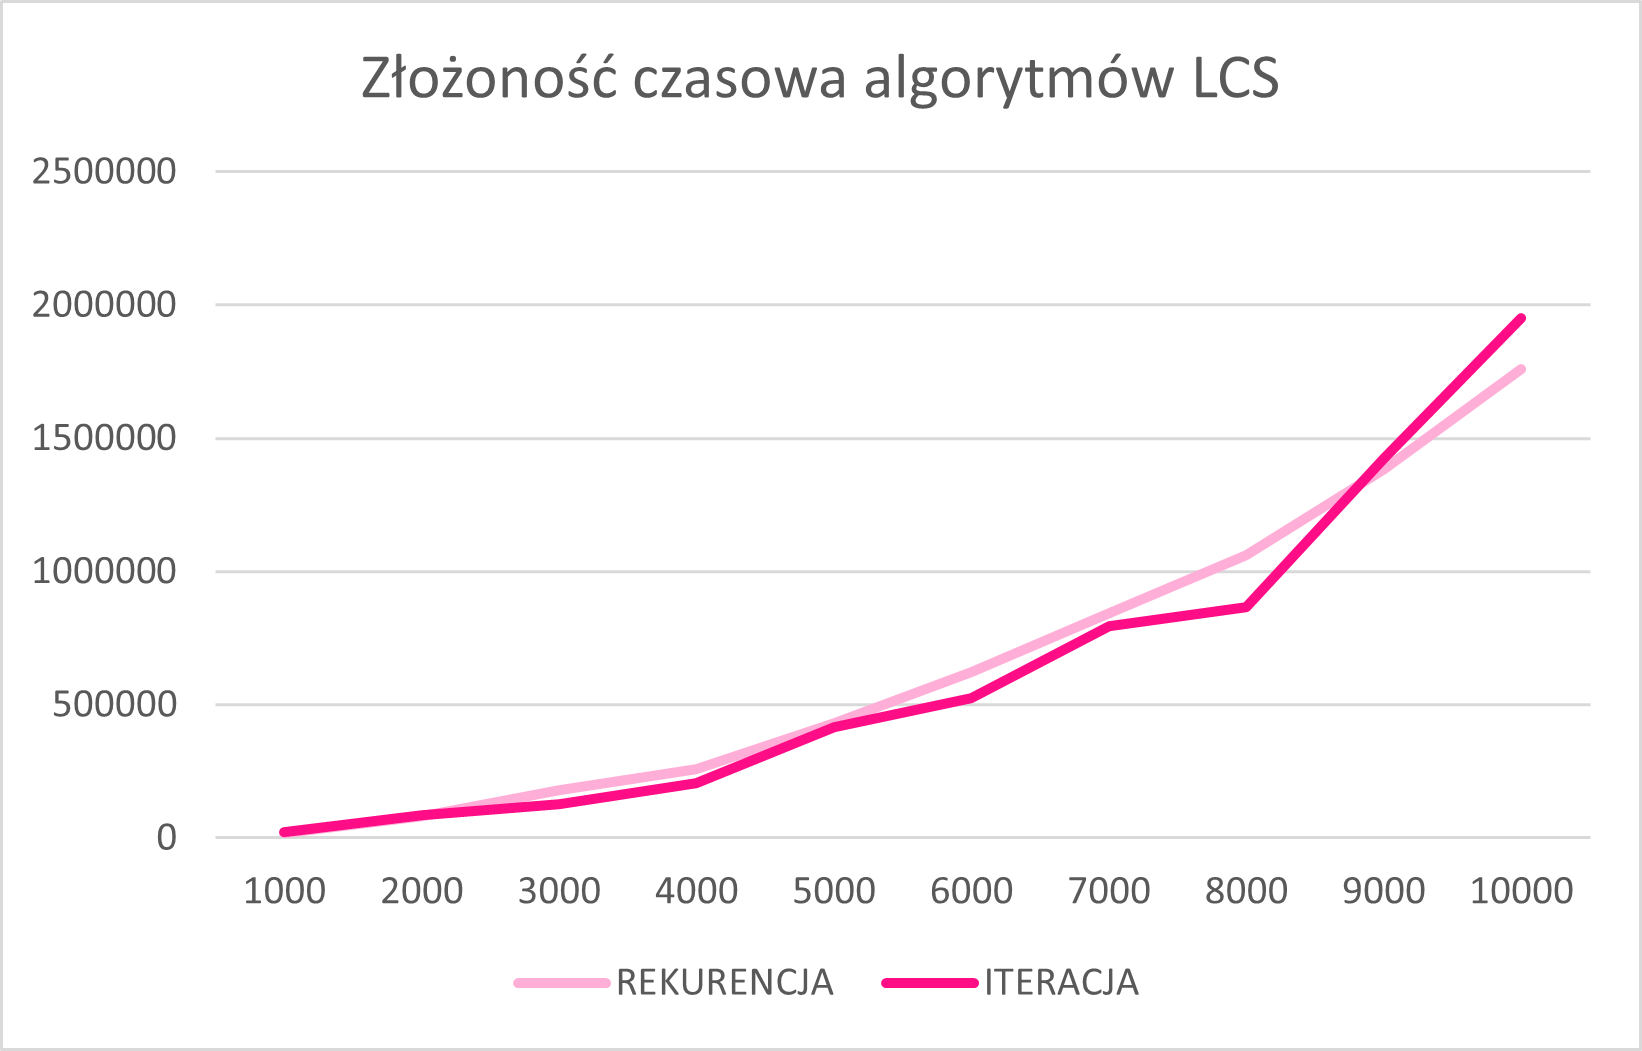
\includegraphics[width = \textwidth]{Obraz2.png}
	\end{center}
	\section*{WNIOSKI}
	Oba algorytmy wykonywały się w bardzo podobnym czasie, bez konkretnego wskazania na przewagę jednego z nich. W większości przypadków wersja z iteracją była szybsza, ale różnice te nie były szczególnie zauważalne, a przewaga ta była niezbyt istotna.
	\subsection*{PORÓWNANIE ALGORYTMÓW WYBORU ZAJĘĆ}
	\begin{center}
		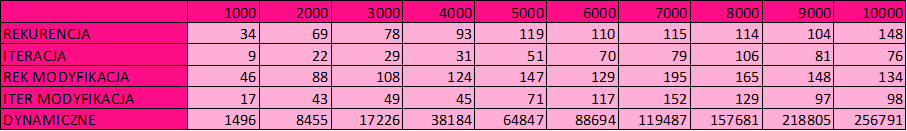
\includegraphics[width = \textwidth]{Obraz5.png}
	\end{center}
	\begin{center}
		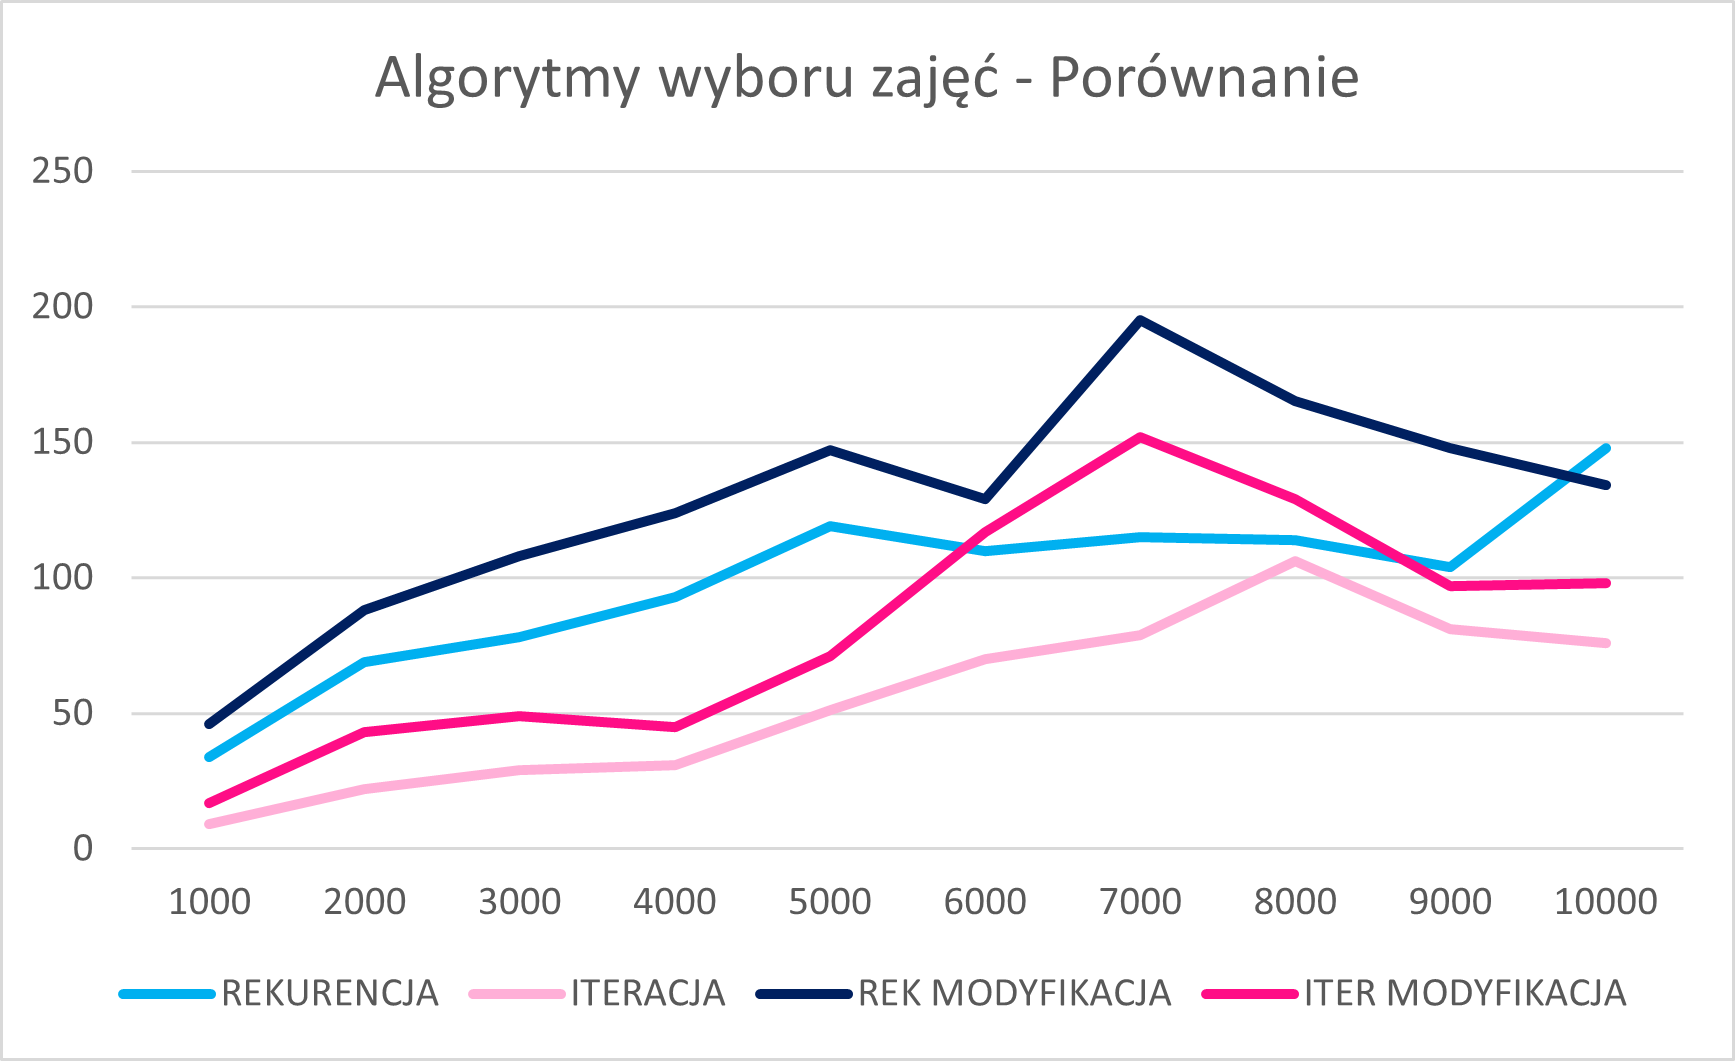
\includegraphics[width = \textwidth]{Obraz4.png}
	\end{center}
	\begin{center}
		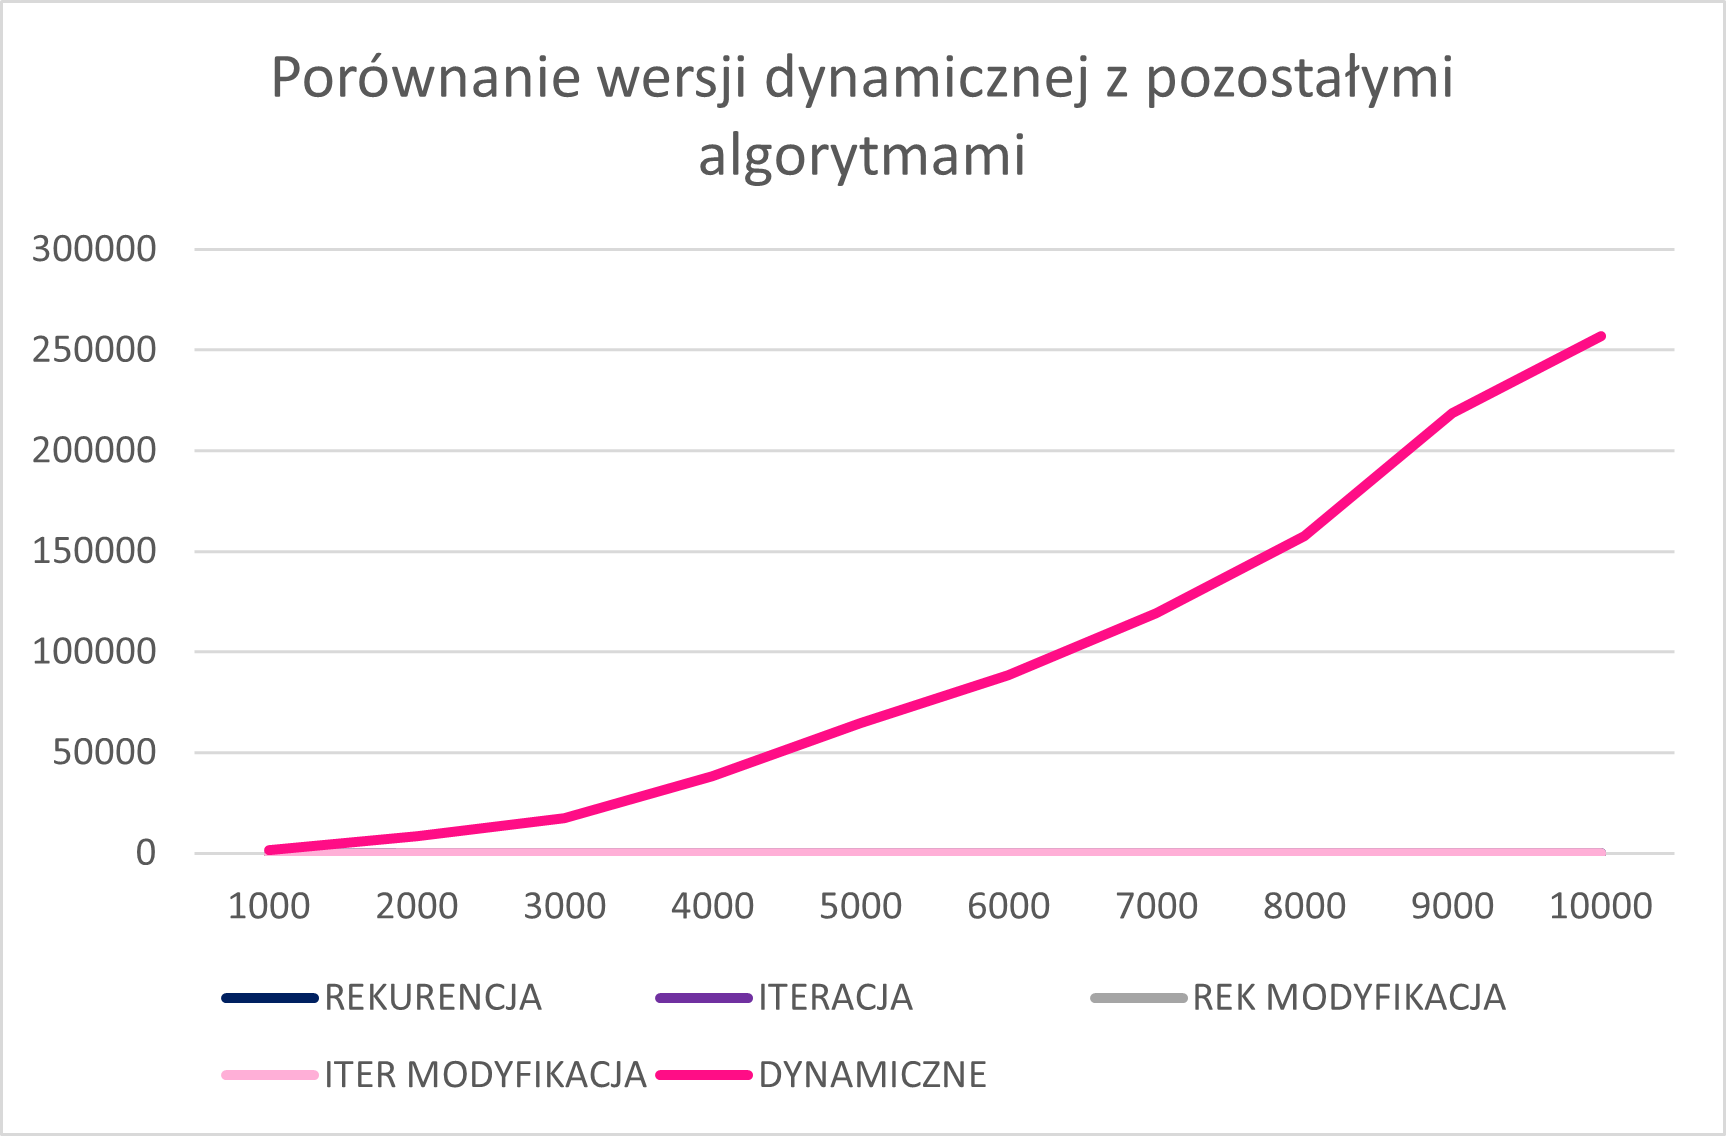
\includegraphics[width = \textwidth]{Obraz1.png}
	\end{center}
	\section*{WNIOSKI}
	Oba podstawowe algorytmy, a także ich modyfikacje wykonywały się bardzo szybko, co spowodowało wahania w wynikach. Nie można zatem zaobserwować szczególnego wydłużenia się czasu wykonywania wraz ze wzrostem długości listy. Nieznacznie szybsza od pozostałych okazała się oryginalna wesja iteracyjna. Porównanie natomiast można wykonać z wersją dynamiczną, która okazała się o wiele bardziej złożona, a czas jej wykonania wyraźnie wzrastał wraz ze wzrostem długości list.
\end{document}
